\section{Audit of the Senior Pipeline and Proposed Method}\label{sec:method}
\subsection{Reproduction and audit}\label{sec:audit}
We ran the released scikit-learn code unchanged on a random sample of real CIC-IoT2023 flows (255{,}000 benign, 245{,}000 DDoS, as in~\cite{senior2026}). The qualitative claims reproduce (17 of 46 features kept; federated equals centralised; Isolation Forest fails, F1 \nv{senior_f1:if}); our federated-SVM F1 is \nv{senior_f1:fed5} against the reported 0.9881, plausibly because the released loader keeps the first rows it meets rather than a random draw. TensorFlow ports of the SVM (F1 \nv{tf:tf_svm_central_hinge} hinge, \nv{tf:tf_svm_central_sqhinge} squared hinge) and of the MLP (\nv{tf:keras_mlp_central}) match scikit-learn (\nv{senior_f1:cent}, \nv{senior_f1:ann}). The audit found four defects that matter for a privacy claim (eight more are in the project's analysis file):
\begin{enumerate}
\item \textbf{Pooled, pre-split preprocessing:} variance filter, Pearson, LDA and scaler are fitted on all rows before \texttt{train\_test\_split}.
\item \textbf{One-shot averaging:} each ``round'' builds a fresh \texttt{LinearSVC} per worker; the global model is never sent back.
\item \textbf{Centralised baselines:} RF, ANN and Isolation Forest are trained centrally although described as federated.
\item \textbf{Loss and duplicates:} squared hinge is used although~\cite{senior2026} lists hinge; \nv{dedup_frac:ciciot}\% of a random sample of the release are exact duplicates that a random split spreads over train and test.
\end{enumerate}

\subsection{Problem formulation}
Client $k\in\{1..K\}$ holds $D_k=\{(x_i,y_i)\}$, $x_i\in\mathrm{R}^d$, $y_i\in\{0,1\}$ (1 = DDoS), $n_k=|D_k|$, $n=\sum_k n_k$. With $\phi(x)=(x_F-m)/s$ (keep features $F$, standardise) and $f_\theta(z)=w^\top z+b$, the goal is
\begin{equation}\label{eq:obj}
\begin{gathered}
\min_\theta F(\theta)=\sum_{k=1}^{K}\frac{n_k}{n}F_k(\theta),\\
F_k(\theta)=\frac1{n_k}\sum_{i\in D_k}\ell\big(y_i,f_\theta(\phi(x_i))\big)+\frac{\lambda}{2}\lVert w\rVert^2 ,
\end{gathered}
\end{equation}
where $\ell$ is the (squared) hinge loss of Eq.~\eqref{eq:loss} and $\lambda=1/(Cn)$ maps a SVM constant $C$ to the mean-loss form. Figs.~\ref{fig:arch} and~\ref{fig:cmp} show the system and its difference from the senior pipeline; Fig.~\ref{fig:models} shows the detectors.

\subsection{FedStat-FS: exact federated preprocessing}
All ingredients of the senior preprocessing (Fig.~\ref{fig:flows}, left) are functions of per-class counts, means and centred second moments, which are additive over clients. In \emph{round A} each client sends
\begin{equation}\label{eq:A}
n_{kc}=\sum_{i\in D_k}\mathrm{I}[y_i=c],\qquad s_{kc}=\sum_{i\in D_k,\,y_i=c}x_i,\quad c\in\{0,1\},
\end{equation}
and the server forms the pooled class counts and means and broadcasts the global mean $\mu$:
\begin{equation}\label{eq:A2}
n_c=\sum_k n_{kc},\ \ \mu_c=\frac{\sum_k s_{kc}}{n_c},\ \ \mu=\frac{n_0\mu_0+n_1\mu_1}{n},\ \ p_1=\frac{n_1}{n}.
\end{equation}
In \emph{round B} each client sends second moments centred at the \emph{global} mean (numerically stable for heavy-tailed byte and packet counts) and the server sums them:
\begin{equation}\label{eq:B}
M_{kc}=\!\!\sum_{i\in D_k,\,y_i=c}\!\!(x_i-\mu)(x_i-\mu)^{\!\top},\qquad M_c=\sum_k M_{kc}.
\end{equation}
The server then obtains the covariance and variance filter~\eqref{eq:var} and the Pearson correlation with the label~\eqref{eq:pear},
\begin{equation}\label{eq:var}
\Sigma=\tfrac1n(M_0+M_1),\quad v_j=\tfrac{(M_0+M_1)_{jj}}{n-1},\quad F_1=\{j:v_j\ge\nu\},
\end{equation}
\begin{equation}\label{eq:pear}
\rho_j=\frac{p_1(\mu_{1j}-\mu_j)}{\sigma_j\sqrt{p_1(1-p_1)}},\qquad F_P=\{j\in F_1:|\rho_j|>\tau\},
\end{equation}
with $\sigma_j^2=\Sigma_{jj}$, because $\mathrm{cov}(x_j,y)=p_1(\mu_{1j}-\mu_j)$. For LDA, the within-class scatter~\eqref{eq:sw} and the discriminant direction on standardised features~\eqref{eq:lda} are
\begin{equation}\label{eq:sw}
S_W=\sum_{c\in\{0,1\}}\big[M_c-n_c(\mu_c-\mu)(\mu_c-\mu)^{\!\top}\big],
\end{equation}
\begin{equation}\label{eq:lda}
w_{\mathrm{LDA}}=D\,S_W^{+}(\mu_1-\mu_0),\qquad D=\mathrm{diag}(\sigma),
\end{equation}
where $S_W^{+}$ is the Moore--Penrose pseudo-inverse and $F_L$ holds the indices of the $k_L$ largest $|w_{\mathrm{LDA}}|$ within $F_1$. The hybrid subset and the global standardiser are
\begin{equation}\label{eq:sel}
F=F_P\cap F_L,\qquad m_j=\mu_j,\ \ s_j=\sigma_j\quad(j\in F).
\end{equation}
Eqs.~\eqref{eq:A}--\eqref{eq:sel} are implemented in \texttt{prep.py} (\texttt{client\_round\_a}, \texttt{client\_round\_b}, \texttt{select\_from\_moments}, \texttt{fit\_federated}). The detector loss and the federated update are
\begin{equation}\label{eq:loss}
\begin{gathered}
\ell_{\mathrm h}=\max(0,1-\tilde y f),\qquad \ell_{\mathrm{sq}}=\ell_{\mathrm h}^{2},\\
H_k(\theta;\theta^t)=F_k(\theta)+\tfrac{\mu_p}{2}\lVert\theta-\theta^t\rVert^2,
\end{gathered}
\end{equation}
\begin{equation}\label{eq:avg}
\theta^{t+1}=\sum_{k=1}^{K}\frac{n_k}{n}\,\theta_k^{t+1},\qquad \theta_k^{t+1}\leftarrow \text{SGD}\big(H_k(\cdot;\theta^t),\theta^t\big),
\end{equation}
with $\tilde y=2y-1$ and $\mu_p=0$ for FedAvg and $\mu_p>0$ for FedProx~\cite{li2020fedprox} (\texttt{models.py}, \texttt{fl.py::fedavg\_svm}). Metrics are accuracy, precision, recall, F1, false-positive rate and the Matthews correlation:
\begin{equation}\label{eq:metrics}
\begin{gathered}
\mathrm{P}=\tfrac{TP}{TP+FP},\ \mathrm{R}=\tfrac{TP}{TP+FN},\ F_1=\tfrac{2\mathrm{PR}}{\mathrm{P}+\mathrm{R}},\ \mathrm{FPR}=\tfrac{FP}{FP+TN},\\
\mathrm{MCC}=\tfrac{TP\,TN-FP\,FN}{\sqrt{(TP{+}FP)(TP{+}FN)(TN{+}FP)(TN{+}FN)}}.
\end{gathered}
\end{equation}
\begin{figure}[t]
\centering
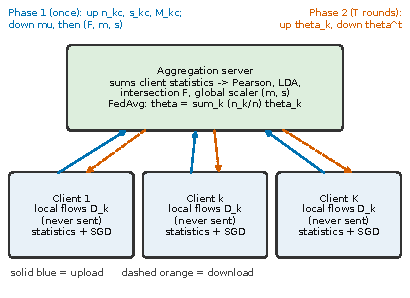
\includegraphics[width=\columnwidth]{d1_system_architecture.pdf}
\caption{System architecture of FedStat-FS: clients never upload rows, only additive statistics (phase 1) and model parameters (phase 2).}
\label{fig:arch}
\end{figure}

\begin{algorithm}[t]
\caption{FedStat-FS and federated linear detector}\label{alg:main}
\begin{algorithmic}[1]
\Require client data $D_k$ (never sent; flowchart in Fig.~\ref{fig:flows}, right), $\nu,\tau,k_L$, rounds $T$, local epochs $E$, step $\eta$, $\lambda$, $\mu_p$
\Ensure approximate minimiser $\theta_T$ of Eq.~\eqref{eq:obj} and $(F,m,s)$
\State clients send $(n_{kc},s_{kc})$ \Comment{Eq.~\eqref{eq:A}}
\State server: $n_c,\mu_c,\mu,p_1$; broadcast $\mu$ \Comment{Eq.~\eqref{eq:A2}}
\State clients send $M_{kc}$ around $\mu$ \Comment{Eq.~\eqref{eq:B}}
\State server: $F_1,F_P,F_L$, $F=F_P\cap F_L$, $(m,s)$; broadcast \Comment{Eqs.~\eqref{eq:var}--\eqref{eq:sel}}
\State $\theta^0\gets 0$
\For{$t=0,\dots,T-1$}
  \State each client: $z_i\gets(x_i[F]-m)/s$; run $E$ SGD epochs on $H_k(\cdot;\theta^t)$ from $\theta^t$
  \State server: $\theta^{t+1}\gets\sum_k \tfrac{n_k}{n}\theta_k^{t+1}$ \Comment{Eq.~\eqref{eq:avg}}
\EndFor
\State \Return $\theta_T,(F,m,s)$
\end{algorithmic}
\textit{Complexity.} Phase 1: client $O(n_kd^2)$ time, $O(d^2)$ memory; server $O(Kd^2+d^3)$. Phase 2 per round: client $O(En_k|F|)$, server $O(K|F|)$; model size $O(|F|)$.
\end{algorithm}
\begin{figure*}[t]
\centering
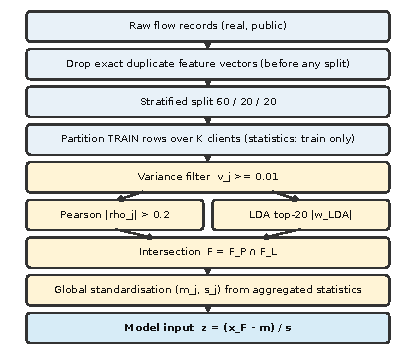
\includegraphics[width=0.485\textwidth]{d3_preprocessing_flowchart.pdf}\hfill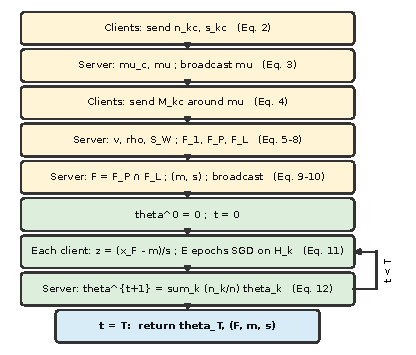
\includegraphics[width=0.485\textwidth]{d6_algorithm_flowchart.pdf}
\caption{Left: preprocessing flowchart (de-duplication and splitting precede every statistic). Right: flowchart of Algorithm~\ref{alg:main}.}
\label{fig:flows}
\end{figure*}
\begin{figure}[t]
\centering
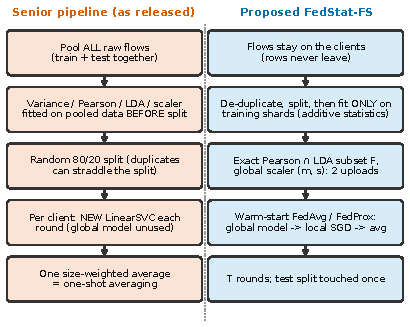
\includegraphics[width=\columnwidth]{d5_senior_vs_proposed.pdf}
\caption{Senior pipeline as released versus FedStat-FS: what was changed.}
\label{fig:cmp}
\end{figure}
\begin{figure*}[t]
\centering
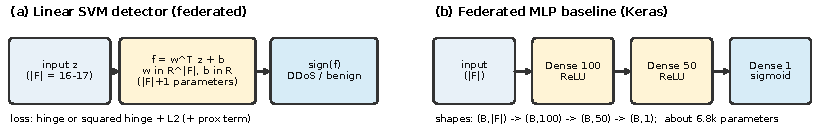
\includegraphics[width=\textwidth]{d4_model_architecture.pdf}
\caption{Detectors: the linear SVM used for federated averaging and the Keras MLP baseline (shapes and parameter counts).}
\label{fig:models}
\end{figure*}
